\documentclass[12pt]{article}
\usepackage{graphicx}
\usepackage{amsmath}
\usepackage{amssymb}
\usepackage[authoryear]{natbib}
\usepackage{enumerate}
\usepackage{booktabs}
\setlength{\parindent}{0pt}
\usepackage[parfill]{parskip}
\date{Lent 2023}
\title{Dissertation draft}
\author{Tobias Leigh-Wood}
\usepackage[letterpaper, margin=1.1in]{geometry}
\linespread{1.1}

\begin{document}
\maketitle


Standard economic theory suggests that retirement annuities should be highly prized by individuals as a way to
insure against the risk of late death \cite{yaari_65}. However, in developed countries rates of annuitization are far below the
levels that theory predicts.
Under the coalition government in the UK the law regarding the use of private defined
contribution pensions changed. Individuals were no longer forced to annuitise their pension pots and could access
them in a variety of ways such as a lump sum withdrawal on retirement or income drawdown and subsequently the number of annuities
sold in the UK dropped precipitously.

I first use the policy reform as a discontintuity to measure the impact of forced annutisation on the consumption
of individuals in the first few years of retirement. Given that the reform was implemented suddenly and without
advanced notice before the Spring 2014 budget I claim that individuals with a retirement year in 2015, 2016 or 2017
are otherwise similar to those with a retirement year in 2011, 2012 and 2013 but the do not need to annuitise their
defined contribution pension pots.


In this paper I test two competing hypotheses for the annuity problem: bequests and
pessimistic life expectancy. Depending on the reason for the lack of annuitization in the UK, the consumption response of retirees to the pension
reform will differ. If individuals do not annuitise because of pessimistic life expectancy I will show that their
consumption should increase. If, on the other hand, individuals do not annuitise because of a bequest motive, consumption
should not change much as a result of the reform. I will solve lifecycle models for both of these cases and simulate
consumption decisions with, and without, forced annuitization. I will then use a variety of empirical models to measure
the consumption change in early retirement that resulted from the policy reform. The size and magnitude of this change
will be indicative of the mechanism causing the annuitization problem.


The importance of retirement policy to individuals in the UK is growing. The number of individuals of
pensionable age is expected to grow from 11.9 million in 2020 to 15.2 million in
2045 according to the latest ONS statistics and for every 1000 people of working age there will be 341 of pensionable
age in 20145 compared to 280 in 2020 \cite{ons_population_predictions_2020}. The increase in absolute and relative
numbers of elderly makes retirement policy more important. Moreover, private, defined contribution (DC), pensions are
becoming increasingly common and are predicted to grow as current cohorts age \cite{cribb_karjalainen_ifs_2023}.
Therefore, policies regarding how private pensions can be accessed will have a larger impact on overall welfare for
retirees.



\subsection{Literature review}
My paper draws on three main strands of literature. The annuity problem, the retirement saving
problem and lifecycle models. \textbf{this intro is rubbish}

\cite{yaari_65} was the first to show that under standard assumptions we would expect individuals to
annuitise all of their wealth at retirement to insure against the risk of long life. Since then there
has been much literature discussing possible reasons that people do not annuitise. \cite{finkelstein_porteba_2002}
and \cite{finkelstein_porteba_2004} find evidence of adverse selection, thereby making the 'money's worth'
of annuities lower for the general population as opposed to the population of annuitants. However, they
also find that theory would still predict annuitization.

\cite{friedman_warshawsky_qje_1990} show that annuitization decisions can be fully explained by a mixture of
bequest motives and actuarily unfair annuities. They solve an augmented life-cycle model with a range of
parameters on how severe the rate of return is on the annuity versus market rates. For plausible values
they find that individuals would optimally not annuitise much wealth. Similarly to \cite{finkelstein_porteba_2004},
\cite{friedman_warshawsky_chicago_1988} show that there is a significant difference between the life expectancy of
annuitants and the general population in the American annuity market but this cannot fully explain the annuitization
problem. Only when bequest motives are added to the model can annuitization rates be rationalized.

\cite{lockwood_red_2012} builds on this and shows that a realistic bequest motive in lifecycle simulations achieves
realistic annuitization rates. He solves a simple lifecycle model with bequest motives taken from several recent papers
in the literature. The bequest motives he picks therefore match other important aspects of the lifecycle model such
as how much individuals actually bequest and how rich individuals are when they bequest.

\cite{lockwood_aer_2018}

\cite{vidalmelia_lejarragagarcia_munich_2004} have some interesting results. Need to talk about that.

\textit{There are some more papers to include here. Time to go and have dinner. }

\section{Data and Policy reform}

\subsection{Data}

The main data set I use is the English Longitudinal Study of Ageing (ELSA) \cite{main_elsa_citation}. ELSA repeatedly interviews
individuals over the age of 50 and asks them a range of questions relating to their income and wealth as well as expectations about
the future. Importantly it also includes detailed information pensions including the type of pension that an individual holds when
working, thus I am able to distinguish between individuals who have defined benefit and defined contribution pensions. For ease of access
I use Harmonized ELSA \footnote{"This analysis uses data or information from the Harmonized ELSA dataset and Codebook, Version G.2 as of
  July 2021 developed by the Gateway to Global Aging Data. The development of the Harmonized ELSA was funded by the National
  Institute on Aging (R01 AG030153, RC2 AG036619, R03 AG043052). For more information,
  please refer to https://g2aging.org/.”} which ensures that variables are comparable across waves. Since this only includes a
subset of the questions in ELSA I also supplement it with variables taken directly from the data.

ELSA also includes questions on expenditures. In particular individuals are asked how much they consume on a range of broad categories.


% Include a summary stats table here of the individuals selected for the regression



I also use life tables from the UK's Office for National Statistics. These give us risk of death for each age group. I adjust them
to make death certain at age 110 as is common in the literature. I transform these so that I have risk of death conditional on being
a given age since this is what is used in the life cycle simulations.
%  include a table showing death probs 



To illustrate the effect the reform had on sales of annuities in the UK I obtained product data from the Financial Conduct Authority.
These track the sale of different financial products overtime including data on annuity sales.


% Plot showing the drop of in annuity sales 

To calculate subjective life expectancies I follow \cite{odea_sturrock_rest_2023}. Individuals are asked “What are the chances that you will
live to be age X or more?” where X changes depending on the age of the interviewee. If individuals were under 65 then X was 75, if individuals
were 66 and older they were asked the age that was 11 to 15 years older than them and is a multiple of 5. From wave three respondents were
also asked “What are the chances that you will live to be age 85 or more?” if they were under 70. As most recent retirees are under 70 we
therefore have two data points. I carry out the following procedures: drop any individuals who think it is more likely they reach an older
age than a younger age since; add, as a third data point their objective chance of reaching 110 according to the ONS life tables; fit these
three points to a Weibull distribution using non-linear least squares. Then I create subjective survival tables.

\textbf{I could go into more detail here? Maybe I should. Add equation etc}

\begin{table}

\caption{Summary statistics \label{tab:sum_stats} }
\centering
\fontsize{10}{12}\selectfont
\begin{tabular}[t]{lrrrrrrrrrr}
\toprule
\multicolumn{1}{c}{ } & \multicolumn{2}{c}{Max} & \multicolumn{2}{c}{Mean} & \multicolumn{2}{c}{Median} & \multicolumn{2}{c}{Min} & \multicolumn{2}{c}{Non Missing} \\
\cmidrule(l{3pt}r{3pt}){2-3} \cmidrule(l{3pt}r{3pt}){4-5} \cmidrule(l{3pt}r{3pt}){6-7} \cmidrule(l{3pt}r{3pt}){8-9} \cmidrule(l{3pt}r{3pt}){10-11}
 & Control & Treat & Control & Treat & Control & Treat & Control & Treat & Control & Treat\\
\midrule
Gender & 1.0 & 1.0 & 0.470 & 0.495 & 0.0 & 0.0 & 0.0 & 0.0 & 753 & 301\\
RetirementYear & 2013.0 & 2017.0 & 2011.875 & 2015.389 & 2012.0 & 2015.0 & 2011.0 & 2015.0 & 753 & 301\\
InterviewYear & 2016.0 & 2017.0 & 2013.328 & 2016.326 & 2014.0 & 2016.0 & 2011.0 & 2015.0 & 753 & 301\\
YearsSinceRetirement & 2.0 & 2.0 & 1.057 & 0.528 & 1.0 & 1.0 & 0.0 & 0.0 & 753 & 301\\
RetiredAge & 82.0 & 79.0 & 63.052 & 63.877 & 63.0 & 64.0 & 55.0 & 55.0 & 753 & 301\\
\addlinespace
AgeAtInterview & 83.0 & 79.0 & 64.109 & 64.405 & 64.0 & 64.0 & 55.0 & 55.0 & 753 & 301\\
ExpectedRetiredAge & 120.0 & 120.0 & 62.317 & 62.773 & 60.0 & 60.0 & 54.0 & 50.0 & 605 & 264\\
DifferenceAge & 48.0 & 44.0 & -0.660 & -0.981 & -1.0 & -1.0 & -8.0 & -22.0 & 605 & 264\\
FinWealth(£000s) & 1.9 & 2.0 & 0.122 & 0.168 & 0.1 & 0.1 & -0.0 & -0.0 & 738 & 297\\
DCPension & 1.0 & 1.0 & 0.198 & 0.259 & 0.0 & 0.0 & 0.0 & 0.0 & 753 & 301\\
\addlinespace
DCValue(£000s) & 8.2 & 17.3 & 0.073 & 0.116 & 0.0 & 0.0 & 0.0 & 0.0 & 684 & 259\\
DBPension & 1.0 & 1.0 & 0.466 & 0.455 & 0.0 & 0.0 & 0.0 & 0.0 & 753 & 301\\
StatePension & 0.0 & 0.0 & 0.005 & 0.005 & 0.0 & 0.0 & 0.0 & 0.0 & 750 & 298\\
OwnsHouse & 1.0 & 1.0 & 0.875 & 0.880 & 1.0 & 1.0 & 0.0 & 0.0 & 753 & 301\\
HouseValue(£000s) & 1.3 & 1.7 & 0.230 & 0.296 & 0.2 & 0.2 & 0.0 & -0.1 & 753 & 301\\
\addlinespace
ObjectiveLifeExp & 33.7 & 34.1 & 23.732 & 23.904 & 23.9 & 23.5 & 7.9 & 10.8 & 753 & 301\\
SubjectiveLifeExp & 36.6 & 37.9 & 20.898 & 20.950 & 21.3 & 21.2 & 4.6 & 5.3 & 527 & 198\\
TotalConsump & 2925.1 & 3495.7 & 729.239 & 780.975 & 647.6 & 699.5 & 130.2 & 136.9 & 753 & 301\\
FoodConsump & 1938.1 & 1938.1 & 415.753 & 425.780 & 363.3 & 373.8 & 51.5 & 36.1 & 748 & 296\\
FoodConsumpIn & 440.0 & 400.0 & 79.964 & 77.706 & 70.0 & 70.0 & 10.0 & 1.0 & 749 & 296\\
\addlinespace
FoodConsumpOut & 750.0 & 1200.0 & 68.302 & 88.208 & 50.0 & 50.0 & 0.0 & 0.0 & 752 & 298\\
ClothingConsump & 1450.0 & 2000.0 & 89.224 & 83.824 & 45.0 & 40.0 & 0.0 & 0.0 & 753 & 301\\
LeisureConsump & 530.0 & 150.0 & 82.072 & 75.000 & 60.0 & 75.0 & 0.0 & 0.0 & 657 & 2\\
UtilityConsump & 483.1 & 580.9 & 107.840 & 113.324 & 96.0 & 100.0 & 0.0 & 0.0 & 753 & 301\\
\bottomrule
\end{tabular}
\end{table}


\subsection{Policy reform}

\textbf{Add some other background to pensions in the UK. What does the Blundell etc have
  to say}

Successive governments in the UK have attempted to reform both the public and private pension system. Prior
to 1987 participation in private schemes was limited to employees of firms that had offered one, and there
were few alternatives to the public state pension or a define benefit scheme that a public sector employee
would offer. \textbf{Were there pension reforms in 1990s and 00s}

Announced in the Spring budge of 2014, the so called "pensions freedom act" received Royal Asset in December 2014 marked the end of a series
of pension reforms carried out by the coalition government between 2010 and 2015. The reform was announced
in the Spring budget and made it possible to withdraw money from a private pension pot subject to the
marginal rate of income tax that an individual faced. In the June 2010 budget the government made a first
reform to the annuitization rules, creating an minimum income requirement above which individuals would not need to
annuitise more \cite{finance_act_hmt_2011}. However, this was set at £20,000 and therefore few individuals
were eligible. The minimum income requirement was scrapped in the 2014 bill finally eliminating the
compulsory annuities market. The impact of the reforms on annuity demand has been documented by \cite{cannon_et_al_nier_2016}.
Using data from the Association of British Insurers they show that annuity demand dropped by 75\% from
its maximum.

After the announcement in spring 2014 sales of annuities dropped massively and income drawdown products increased.
However, pension pots could also be taken out in one go and this became a much more common option for many people.

Figure \ref{fig:annovertime} shows purchases of annuities overtime and demonstrates the sharp decrease
in purchases that happened from 2014 to 2015. Likewise there was an increase in the number of pensions that were
being accessed using an income drawdown product, but these do not fully account for the drop in annuitisation. So,
either they are withdrawn at once or they are left alone.

Figure \ref{fig:ann2122} shows the current distribution of how pension pots are first accessed at retirement.
In 2021, 196,736 pots were fully withdrawn at retirement, accounting for over 50\% of pots, prior to the policy
reform this was not the case and most defined contribution pensions were accessed through annuities.


\begin{figure}[h]
  \caption{Pension pots accessed}
  \centering
  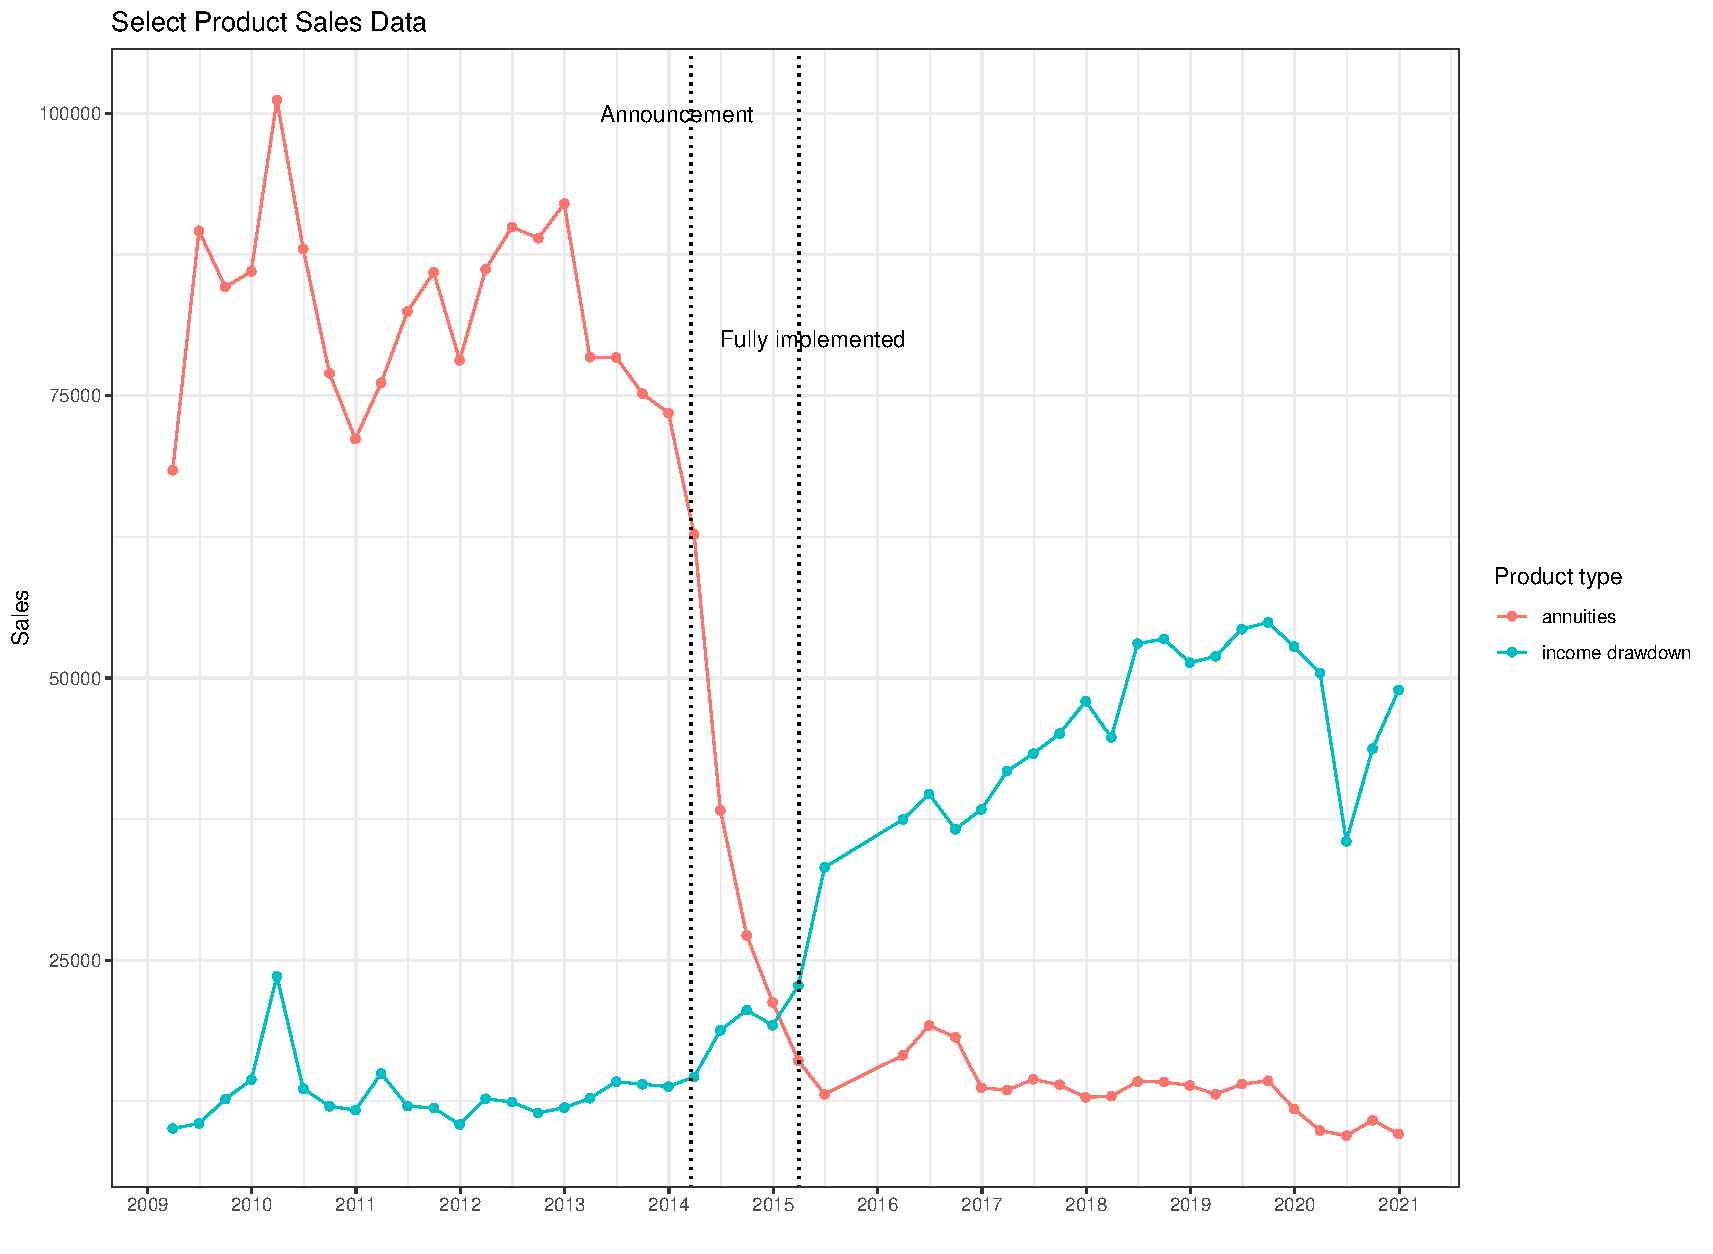
\includegraphics[width=0.7\columnwidth]{figures/annuity_overtime.pdf}
  \label{fig:annovertime}
\end{figure}

\begin{figure}[h]
  \caption{How pension pots are accessed}
  \centering
  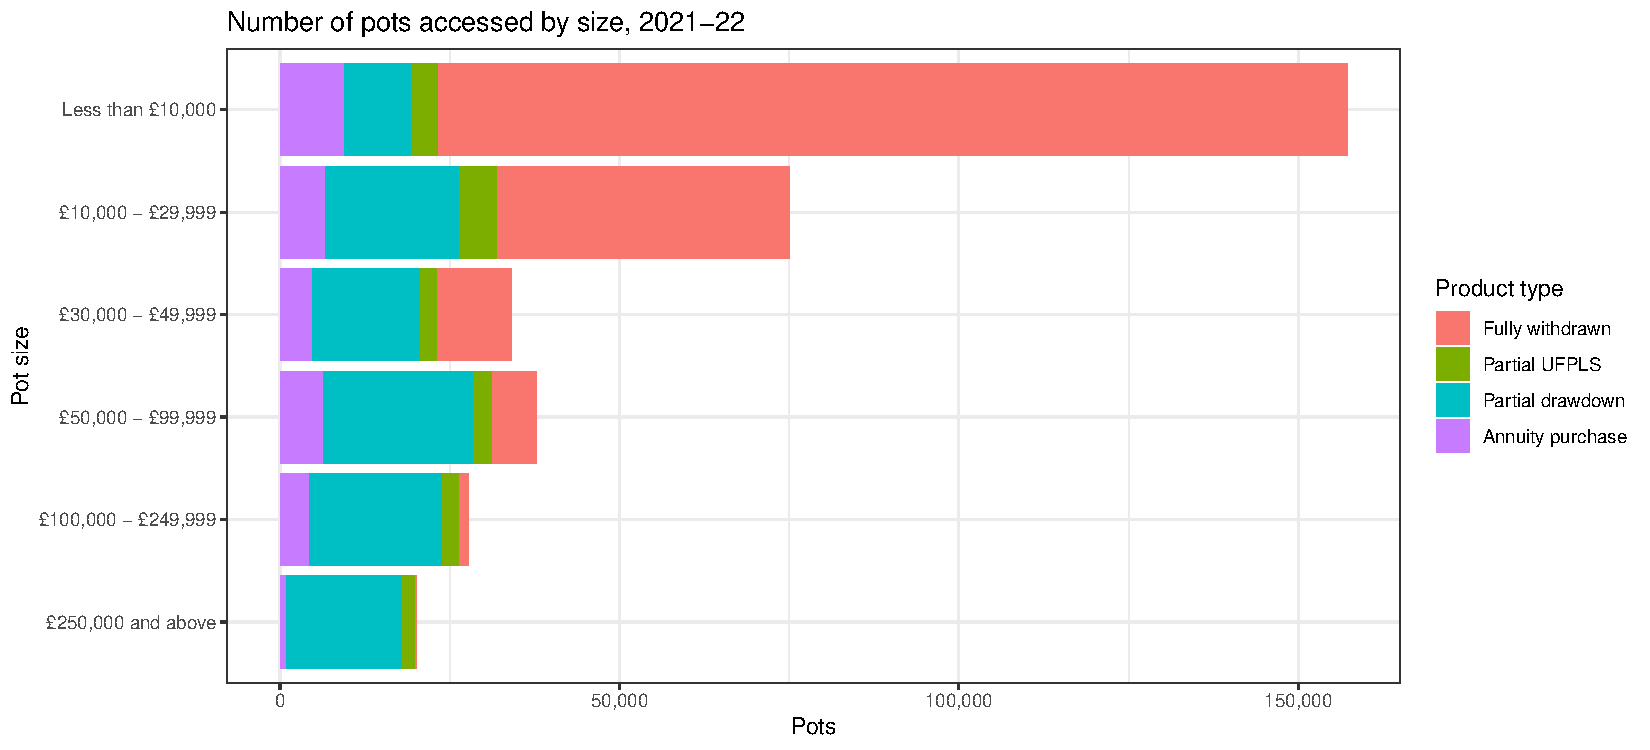
\includegraphics[width=0.7\columnwidth]{figures/annuity_pot_sizes.pdf}
  \label{fig:ann2122}
\end{figure}


\subsection{Covariate Balance}

I regress demographic and financial characteristics of individuals on year of birth and the treatment dummy.
We can then see if the treatment groups differ on key characteristics such as financial wealth or retirement age.
For a regression discontinuity to be valid we need the treatment and control groups to be similar along
all other characteristics apart from the treatment variable.

In particular I run:
\begin{equation*}
  Y_{i} = \alpha + \beta Post_{i} + \gamma YOB + \kappa (Post_{i} \times YOB_{i}) + \epsilon_{i}
\end{equation*}

\begin{table}

\caption{Covariate Balance \label{tab:cov_balance}}
\centering
\begin{tabular}[t]{lll}
\toprule
 & Pt. est. & SE\\
\midrule
Gender & 2.243 & 10.468\\
RetirementYear & -12.528 & 16.127\\
InterviewYear & -11.243 & 24.959\\
YearsSinceRetirement & 9.716 & 16.056\\
RetiredAge & -12.528 & 16.127\\
\addlinespace
ExpectedRetiredAge & -240.427 & 129.345\\
DifferenceAge & -246.763 & 128.979\\
FinancialWealth (thousands) & -4769.638 & 5410.054\\
DCPension & -13.608 & 8.933\\
DCValue (thousands) & -1978.144 & 20284.768\\
\addlinespace
DBPension & 7.974 & 10.386\\
OwnsHouse & -0.697 & 6.968\\
HouseValue (thousands) & 6630.186 & 4775.236\\
ObjectiveLifeExp & 13.086 & 30.559\\
SubjectiveLifeExp & 0.351 & 182.705\\
\bottomrule
\end{tabular}
\end{table}

Table \ref{tab:cov_balance} shows these results. We can see ...


Another threat to validity is manipulation of the running variable. This is probably quite a threat in our case
as individuals could delay retirement and/or the purchase of an annuity.


\section{Methodology and Econometric Strategy}

I first solve a modified retirement lifecycle model. The problem that retirees face is as follows.
Every period retirees solve:
\begin{equation*}
  V_{t}(a_{t}, y) = \underset{a_{t+1}, c_{t}}{\max} \{ u(c_{t}) + p_{t}B(a_{t+1}) + \beta(1-p_{t})V_{t+1}(a_{t+1}, y) \}
\end{equation*}
subject to their budget constraint
\begin{equation*}
  c_{t} =a_{
  t}(1 +r) -  a_{t+1} + y
\end{equation*}
where $a_{t}$ are asset holdings in time t, $y$ is constant income for all periods and . Income can come either
from state pensions, defined benefit pension plans or purchased annuities.
\begin{equation*}
  u(c_{t}) = \frac{c_{t}^{1 - \sigma}}{1 - \sigma}
\end{equation*} In some specifications retirees can leave bequests, I use the bequest function from
\cite{lockwood_red_2012}.
\begin{equation*}
  B(a_{t}) = \bigl( \frac{m}{1 - m} \bigr)^{\sigma}  \frac{(\frac{m}{1 - m}c_{0} + a_{t})^{(1 - \sigma)}}{1 - \sigma}
\end{equation*}
Where $b_{t}$ is the amount left at death, $m$ is a measure of bequest motive strength and $c_{0}$ is
a minimum amount of consumption that individuals want. \textbf{Check this}

First, I discretise the state space. I create a grid from 500 to 50,000 incrementing by 500 for income and 1000 to
500,000 incrementing by 1000 for financial assets. I solve the retirees problem using backward induction. At age 110 there is certainty of death so any leftover assets
are carried over into the next period and bequested. This means that the value at the end of the final period is
either 0 (if we do not allow a bequest motive) or the value of bequests. I then take this value function and solve
an individuals final period problem, choosing assets next period (i.e. those to bequest) and how much to consume.

Using the optimal policy function in the last period, I calculate the value of the last period, which the utility
function and the value function evaluated at the maximum. This is then used in the problem the year before that.
I repeat this process back to the age of retirement to obtain optimal consumption amounts for each year of retirement
and associated value functions.

To simulate the ELSA data I solve this retirement problems for each new retiree in the data set dependent on their
objective probability of death each period. I estimate with subjective life expectancies and objective life expectancies,
I also estimate the model both with and without a bequest motive which was picked to fit the unforced real annuity
rates seen in the data. I then estimate several empirical models with the simulated data.

In retirees first year of retirement I allow them to choose to annuitise some of their wealth. In practical terms
this is moving down the asset grid but up the income grid and seeing if the value of being in that position is better
than where the individual is currently. To calculate this trade-off I calculate the annual annuity payment that follows
from a given annuity cost. I calculate this using objective life tables from the ONS using the following equation:

\begin{equation*}
  Ann = \delta * C * \biggl[\sum_{t = Retage}^{110}\frac{1 - p_{t|Retage}}{(1 + r)^{t - Retage}}\biggr]^{-1}
\end{equation*}

Where $C$ is the one-off payment, $\delta$ is a factor that controls the 'money's worth' of annuity and $p_{t|Retage}$
is the probability of death at age $t$ conditional on being age $Retage$. So individuals can move C on the asset grid
for gaining Ann on the income grid for the rest of their lives.

\section{Empirical models}

In this section I outline the key empirical models I run with both the simulated consumption data from the
lifecycle models and with the real data from ELSA. I then see which lifecycle model better fits the consumption
response that happened as a result of the pension reform.

I use a regression discontinuity design where I compare the consumption of recent retirees after the policy reform
to recent retirees before the policy reform. The individuals who retired in 2014 and later were not forced to
annuitise their defined contribution pension. The key assumption implicit in regression discontinuities is
that nothing else changes at the time of the jump apart from the policy of interest. And that the policy occurs
without individuals predicting it. The policy change was widely seen as a surprise by the media and financial planners,
some of whom in fact complained that they had not been consulted enough. \textbf{How can I justify no other jumps at the jump}

Retirement year is the running variable and individuals are treated if retirement year is greater than 2013 and less than 2016.
I consumption of individuals up to 2 years into retirement so that the sample size is larger. So if someone retired in 2014 and
had consumption data in 2014 and 2016 I include both values. An individual is considered not treated if they retire before 2013 and after 2011.
One benefit of using ELSA is that it includes data on pension type for individuals who are working. Therefore, I can differentiate
between individuals who have a defined contribution pension and those who have a defined benefit contribution. To account for the fact
that the reform only impacted individuals who had accumulated defined contribution pension pots I interact the treatment dummy with
an indicator variable signalling whether the individual had ever held a DC pension pot.

The estimating equation is therefore

\begin{equation*}
  Cons_{it} =  \gamma X_{it} + \beta PostReformDC_{it} + \epsilon
\end{equation*}

And $X_{it}$ is a set of controls including financial wealth etc

I also run the regression with a variety of consumption variables.

I also simulate the expected change in consumption given forced annuitisation and no annuitisation.
The benefit of simulating an individuals decision is that we can directly compare what they would have
consumed with what they actually consumed.

\subsection{Rough plan}
\begin{itemize}
  \item Intro
        \begin{enumerate}
          \item I think Eric French wrote something about population that I could use in then intro to say why it is important.
          \item "Latest data from HM Revenue Customs (published in April) showed more than £45bn has been taken from pots since 2015."
                https://www.ftadviser.com/pensions/2022/02/08/pension-freedoms-were-they-really-a-good-idea/


          \item Add bit about DC/DB pensions in the intro. Also talk about heterogeneity across countries.
                Some countries want to move towards more annuitisation. This annual review is a good source of info
                \cite{banks_crawford_ar_2022}
        \end{enumerate}
  \item Lit review
  \item Models
  \item Empirical
        \begin{enumerate}
          \item Diff in diff
          \item RDD
          \item Matching?
          \item can I use anything I learnt in panel?
                In some sense the decision to annuitise is a discrete choice problem so I could use something from there.
        \end{enumerate}
  \item Conclusion
\end{itemize}


\bibliographystyle{chicago}
\bibliography{references}
\end{document}